\chapter{Diseño e implementación} % Main chapter title

\label{Chapter3} % Change X to a consecutive number; for referencing this chapter elsewhere, use \ref{ChapterX}

\definecolor{mygreen}{rgb}{0,0.6,0}
\definecolor{mygray}{rgb}{0.5,0.5,0.5}
\definecolor{mymauve}{rgb}{0.58,0,0.82}

%%%%%%%%%%%%%%%%%%%%%%%%%%%%%%%%%%%%%%%%%%%%%%%%%%%%%%%%%%%%%%%%%%%%%%%%%%%%%
% parámetros para configurar el formato del código en los entornos lstlisting
%%%%%%%%%%%%%%%%%%%%%%%%%%%%%%%%%%%%%%%%%%%%%%%%%%%%%%%%%%%%%%%%%%%%%%%%%%%%%
\lstset{ %
  backgroundcolor=\color{white},   % choose the background color; you must add \usepackage{color} or \usepackage{xcolor}
  basicstyle=\footnotesize,        % the size of the fonts that are used for the code
  breakatwhitespace=false,         % sets if automatic breaks should only happen at whitespace
  breaklines=true,                 % sets automatic line breaking
  captionpos=b,                    % sets the caption-position to bottom
  commentstyle=\color{mygreen},    % comment style
  deletekeywords={...},            % if you want to delete keywords from the given language
  %escapeinside={\%*}{*)},          % if you want to add LaTeX within your code
  %extendedchars=true,              % lets you use non-ASCII characters; for 8-bits encodings only, does not work with UTF-8
  %frame=single,	                % adds a frame around the code
  keepspaces=true,                 % keeps spaces in text, useful for keeping indentation of code (possibly needs columns=flexible)
  keywordstyle=\color{blue},       % keyword style
  language=[ANSI]C,                % the language of the code
  %otherkeywords={*,...},           % if you want to add more keywords to the set
  numbers=left,                    % where to put the line-numbers; possible values are (none, left, right)
  numbersep=5pt,                   % how far the line-numbers are from the code
  numberstyle=\tiny\color{mygray}, % the style that is used for the line-numbers
  rulecolor=\color{black},         % if not set, the frame-color may be changed on line-breaks within not-black text (e.g. comments (green here))
  showspaces=false,                % show spaces everywhere adding particular underscores; it overrides 'showstringspaces'
  showstringspaces=false,          % underline spaces within strings only
  showtabs=false,                  % show tabs within strings adding particular underscores
  stepnumber=1,                    % the step between two line-numbers. If it's 1, each line will be numbered
  stringstyle=\color{mymauve},     % string literal style
  tabsize=2,	                   % sets default tabsize to 2 spaces
  title=\lstname,                  % show the filename of files included with \lstinputlisting; also try caption instead of title
  morecomment=[s]{/*}{*/}
}


%----------------------------------------------------------------------------------------
%	SECTION 1
%----------------------------------------------------------------------------------------
En este capítulo se detallan los componentes realizados por el autor de esta memoria.
Se explica como se crearon los servicios y como se interconectaron para lograr que todo funcione como una única solución.

\section{Arquitectura y orquestación}
\label{ch3Arq}
Esta sección trata sobre la conexión entre los servicios del trabajo y su despliegue automático.

Para planificar la orquestación se analizaron los servicios que debían ser accesibles desde entidades externas al servidor.
En la figura \ref{fig:ch3EsquemaTrabajo} se pueden observar las conexiones lógicas entre los contenedores.
Destacadas en color rojo, se encuentran las entidades externas que interactúan con el servidor Nodos.
Las interconexiones se simplificaron al crear una capa de puente de red que corre sobre el \emph{Daemon} de Docker.
El resultado es que cada contenedor pasa a tener una dirección de ip dentro del entorno.
La creación de la red se logró con el código \ref{cod:dcNetwork}.

\begin{figure}[h]
	\centering
	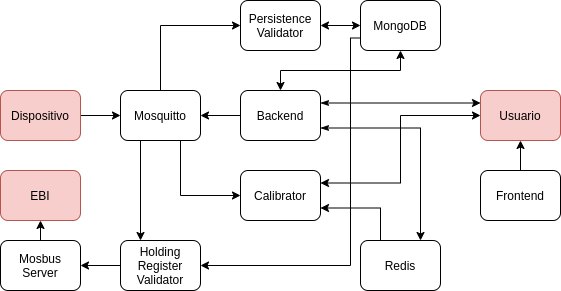
\includegraphics[width=\textwidth]{./Figures/ch3EsquemaTrabajo.png}
	\caption{Esquema de conexión de los servicios.}
	\label{fig:ch3EsquemaTrabajo}
\end{figure}

\begin{lstlisting}[label=cod:dcNetwork,caption=Red de interconexión Docker Compose.]
networks: 
	iot:
		driver: bridge
\end{lstlisting}

\subsection{Servidor Modbus}

El servicio modbus-server se comunica al exterior utilizando el puerto 502.
El puerto pertenece a la lista de protocolos bien conocidos o puertos de sistema.
Esta condición hace posible que existan problemas con los permisos que el usuario tiene dentro del sistema operativo.
Como se puede observar en el código \ref{cod:dcModbusServer}, se conectó el puerto 502 del ordenador con el 5020 dentro de la red de Docker.
En general, es una buena práctica que los puertos internos de la red no sean puertos de sistema para no generar conflictos de permisos y conectarlos a puertos de protocolos según sea necesario.
Para evitar usar direcciones ip en el código de los servicios se utilizó el parámetro hostname para utilizar el servicio de sistema de nombres de dominio (DNS) que corre dentro del \emph{Daemon} de Docker.

\begin{lstlisting}[label=cod:dcModbusServer,caption=Orquestación del servidor Modbus.]
modbus-server:
	image: oitc/modbus-server
	container_name: modbus-server
	hostname: modbus-server
	restart: always
	ports:
		- '502:5020'
	expose: 
    	- '5020'
	networks: 
		- iot
\end{lstlisting}

\subsection{Broker Mosquitto}

El servicio Mosquitto se configuró con tres volúmenes que conectan al contenedor con archivos no efímeros que persisten la información.
De esta manera se asegura que el contenedor muestre un comportamiento correcto.
Como se puede apreciar en el código \ref{cod:dcMosquitto}, se encuentran los archivos de configuración de usuarios y de lista de control de acceso (acl).
Con esta configuración se evita que dispositivos anónimos puedan utilizar el broker y que además solo se puedan utilizar los \emph{topics} designados.
Adicionalmente, los distintos usuarios tienen diferentes permisos según el \emph{topic}.
Así se logra una mayor confiabilidad y seguridad en el manejo de los mensajes.

\begin{lstlisting}[label=cod:dcMosquitto,caption=Orquestación del broker Mosquitto.]
mosquitto:
	image: eclipse-mosquitto
	container_name: mosquitto
	hostname: mosquitto
	restart: always
	volumes: 
		- ./mosquitto/mosquitto.conf:/mosquitto/config/mosquitto.conf
		- ./mosquitto/users.txt:/mosquitto/config/users.txt
		- ./mosquitto/acl.txt:/mosquitto/config/acl.txt
	expose: 
		- '1883'
		- '9001'
	ports: 
		- '1883:1883'
		- '9001:9001'
	networks: 
		- iot
\end{lstlisting}

\subsection{Validación de registros Modbus}

El servicio Holding Registers Validator (hrv) tiene la particularidad de depender de otros servicios, como se puede ver en el cógigo \ref{cod:dcHRV}.
El contenedor no puede ser creado hasta que los servicios listados como dependencias se encuentren activos.
Esto se hace de esta manera para evitar que el contenedor genere excepciones y se reinicie varias veces durante el despliegue se la solución.
Además no es posible saber si el comportamiento final del contenedor puede quedar indefinido.
Es importante mencionar que este servicio no tiene salida al exterior y no queda visible por la falta de campos \emph{ports}.

La imagen para construir el contenedor no existe y debe ser creada al momento del despliegue.
Para lograrlo se utiliza el campo \emph{build}, en donde se especifica la ruta al Dockerfile que contiene la receta.
La imagen queda guardada con el nombre vaca/hrv, de esta manera, no es necesario volver a construirla si se decide reiniciar la aplicación.

\begin{lstlisting}[label=cod:dcHRV,caption=Orquestación del servicio hrv.]
hrv:
	build: ./holdingRegistersValidator/
	image: vaca/hrv
	container_name: hrv
	hostname: hrv
	restart: always
	expose: 
		- '1883'
		- '5020'
	depends_on: 
		- 'mosquitto'
		- 'mongo'
		- 'modbus-server'
	networks: 
		- iot
\end{lstlisting}

El Dockerfile que fabrica la imagen puede verse en el código \ref{cod:dfHRV}.
Este código es común para todos los Dockerfiles que construyen imágenes para los servicios realizados en Python.
Se utiliza Alpine Linux como imagen base y se genera el usuario y grupo \emph{pythonuser}.
El usuario es quien corre el servicio dentro del contenedor y se definió un comando a ejecutar al momento de crearlo.
Quedan indicados en este archivo cuales son puertos que se pueden usar para la red puente.

\begin{lstlisting}[language=bash,label=cod:dfHRV,caption=Dockerfile del servicio hrv.]
FROM python:3.8-alpine
LABEL maintainer="Gonzalo Nahuel Vaca <vacagonzalo@gmail.com>"
RUN addgroup -g 1000 -S pythonuser && \
	adduser -u 1000 -S pythonuser -G pythonuser && \
	mkdir -p /app && \
	pip3 install pyModbusTCP && \
	pip3 install paho-mqtt && \
	pip3 install pymongo
ADD --chown=root:root app/* /app/
USER pythonuser
EXPOSE 1883 27017 5020/tcp
CMD [ "python", "-u", "/app/service.py" ]
\end{lstlisting}

\subsection{MongoDB}

El servicio MongoDB no tiene salida al exterior del servidor y su configuración se puede ver en el código \ref{cod:dcMongo}.
La configuración tiene la particularidad de introducir un comando a la hora de crear el contenedor.
Así se le indica al motor de MongoDB cual puerto debe escuchar.
Además se crea un volumen donde figuran una serie de archivos que pueblan la base de datos con información para construir una maqueta.
Esta maqueta fue utilizada para realizar la demostración al cliente.
Los archivos son devices.js, measurements.js, seed.js y users.js.
El archivo devices.js crea una serie de dispositivos ficticios.
El archivo measurements.js inserta una serie de mediciones que provienen de los dispositivos ficticios creados por devices.js.
El script users.js genera una serie de usuarios con distintos permisos, con el fin de probar la capacidad de autentificar las sesiones.
Finalmente seed.js es quién carga todos los datos en MongoDB.
Según se puede ver en el código \ref{cod:dcSeed}, las mediciones fueron cargadas múltiples veces para generar un volumen de datos que sirviera para realizar pruebas.

\begin{lstlisting}[label=cod:dcMongo,caption=Orquestación de MongoDB.]
mongo:
	image: mongo
	container_name: mongo
	hostname: mongo
	command: mongod --bind_ip_all --port 27017
	expose: 
		- '27017'
	volumes: 
		- ./mongodb/scripts:/scripts
	networks:
		- iot
\end{lstlisting}

\begin{lstlisting}[label=cod:dcSeed,caption=Seed de la base de datos.]
use gador;
load("scripts/devices.js")
load("scripts/users.js")
load("scripts/measurements.js")
load("scripts/measurements.js")
load("scripts/measurements.js")
load("scripts/measurements.js")
load("scripts/measurements.js")
load("scripts/measurements.js")
load("scripts/measurements.js")
load("scripts/measurements.js")
load("scripts/measurements.js")
\end{lstlisting}

\subsection{Validación de mediciones}

El servicio Persistence Validator (pv) está definido en el código \ref{cod:dcPV} y se puede observar que la imagen no existe.
Debe ser construida utilizando un Dockerfile.
Como el servicio fue realizado en Python, el Dockerfile necesario para construir la imagen es prácticamente idéntico al visto en el código \ref{cod:dfHRV}.

\newpage

\begin{lstlisting}[label=cod:dcPV,caption=Orquestación del servicio pv.]
	pv:
		build: ./persistenceValidator
		image: vaca/pv
		container_name: pv
		hostname: pv
		restart: always
	expose: 
		- '1883'
		- '27017'
	depends_on: 
		- 'mosquitto'
		- 'mongo'
	networks: 
		- iot
\end{lstlisting}

\subsection{Backend}

Para orquestar el servicio backend, según el código \ref{cod:dcBackend}, se utilizó el puerto 8080 del ordenador para permitir la comunicación con una entidad externa.
La imagen para crear el contenedor debe ser construida y para tal fin se usó el Dockerfile que se puede observar en el código \ref{cod:dfBackend}.
El Dockerfile parte de la imagen oficial de Nodejs y copia los archivos de dependencias dentro del contenedor auxiliar.
Con este contenedor se descargan las bibliotecas necesarias.
Luego se copia el código fuente de la aplicación y finalmente se configura la inicialización del servidor Nodejs como comando por defecto.

\begin{lstlisting}[label=cod:dcBackend,caption=Orquestación del servicio Backend.]
backend:
	build: ./backend
	image: vaca/backend
	container_name: backend
	hostname: backend
	expose: 
		- '1883'
		- '6379'
		- '27017'
	ports: 
		- '8080:8080'
	depends_on:
		- 'mosquitto' 
		- 'mongo'
		- 'redis'
	networks: 
		- iot
\end{lstlisting}

\begin{lstlisting}[language=bash,label=cod:dfBackend,caption=Dockerfile del servicio Backend.]
FROM node
LABEL maintainer="Gonzalo Nahuel Vaca <vacagonzalo@gmail.com>"
WORKDIR /usr/src/app
COPY package*.json ./
RUN npm install
COPY . .
EXPOSE 1883 6379 8080 27017
CMD ["node", "./src/app.js"]
\end{lstlisting}

\subsection{Servicio de calibración}

El servicio Calibrator es una aplicación de Nodejs y fue orquestada de manera similar al servicio Backend.
Su configuración se puede observar en el código \ref{cod:dcCalibrator}.
El Dockerfile necesario para crear su imagen es prácticamente idéntico al mostrado en el código \ref{cod:dfBackend}.

\begin{lstlisting}[label=cod:dcCalibrator,caption=Orquestación del servicio Calibrator.]
calibrator:
	build: ./calibrator
	image: vaca/calibrator
	container_name: calibrator
	hostname: calibrator
	expose: 
		- '1883'
		- '9999'
	ports:
		- '9999:9999'
	depends_on: 
		- 'mosquitto'
	networks: 
		- iot
\end{lstlisting}

\subsection{Redis}

El servicio Redis fue creado a partir de la imagen oficial de Redis que se encuentra disponible en Dockerhub. \citep{contrib:redis}
Como no tiene exposición al exterior del servidor, no se necesitó realizar ninguna configuración adicional.
Es importante aclarar que si bien se puede aplicar una capa de seguridad, no es aconsejable exponer a Redis a la Internet.
La orquestación se puede ver en el código \ref{cod:dcRedis}.

\begin{lstlisting}[label=cod:dcRedis,caption=Orquestación del servicio Redis.]
redis:
	image: redis
	container_name: redis
	hostname: redis
	expose:
		- '6379'
	networks: 
		- iot
\end{lstlisting}

\subsection{Frontend}

El último servicio es el Frontend que fue orquestado como se puede observar en el código \ref{cod:dcFrontend}.
Su imagen se crea usando el código fuente de la aplicación y un Dockerfile al momento de orquestar la solución.
La construcción de esta imagen es la más sofisticada de todo el trabajo, como se puede ver en el código \ref{cod:dfFrontend}.

\begin{lstlisting}[label=cod:dcFrontend,caption=Orquestación del servicio Frontend.]
frontend:
	build: ./frontend/
	image: vaca/frontend
	container_name: frontend
	hostname: frontend
	restart: always
	ports: 
		- '80:80'
\end{lstlisting}

El Dockerfile se divide en dos grandes etapas.
La primer parte es crear un contenedor auxiliar a partir de la imagen oficial de Nodejs y llamarla \emph{builder}.
Este contenedor temporal copia dentro suyo el código fuente del servicio e instala todas las dependencias.
Entre las dependencias instaladas se encuentra el framework de Angular.
Se utiliza el framework para compilar el código fuente de TypeScript y se obtienen archivos en JavaScript que son ejecutables por un navegador.
La segunda parte del proceso es crear un contenedor a partir de la imagen oficial de Nginx, que es un servidor web.
Se transfieren los archivos compilados por el contenedor auxiliar hacia el contenedor de Nginx y se destruye el auxiliar.
Finalmente se transforma el contenedor de Nginx con los archivos compilados en una imagen.

\begin{lstlisting}[language=bash,label=cod:dfFrontend,caption=Dockerfile del servicio Frontend.]
FROM node as builder
WORKDIR /src/app
COPY . ./
RUN npm install
RUN npm run ng build  --prod
FROM nginx
COPY --from=builder /src/app/dist/frontend /usr/share/nginx/html
\end{lstlisting}

\subsection{Despliegue automático}

Con los Dockerfiles definidos y el archivo docker-compose.yml se puede utilizar un guión escrito en Bash que lanza la aplicación.
Como se puede observar en el código \ref{cod:bashStart}.

Cuando se desea eliminar todo rastro del sistema del ordenador, se puede utilizar el código \ref{cod:bashClean}.

Los únicos requisitos para iniciar la aplicación es tener un ordenador que tenga Docker y Docker Compose instalados.
No se necesita tener ninguna de las herramientas de desarrollo dentro del ambiente de producción.
De esta manera se logró una solución altamente portátil y agnóstica de la arquitectura del hardware.

\begin{lstlisting}[language=bash,label=cod:bashStart,caption=Guión de inicialización.]
#!/bin/bash
chmod +x clean.sh
docker-compose up -d
printf "Waiting 10 seconds for internal connections to be made"
sleep 10
docker-compose exec mongo sh -c "mongo < /scripts/seed.js"
printf "checking collections"
docker-compose exec mongo sh -c "mongo < /scripts/seed.test.js"
\end{lstlisting}

\begin{lstlisting}[language=bash,label=cod:bashClean,caption=Guión de limpieza.]
#!/bin/bash
docker-compose down
docker rmi vaca/backend
docker rmi vaca/hrv
docker rmi vaca/pv
docker rmi vaca/auth-api
docker rmi vaca/calibrator
docker rmi vaca/frontend
clear
\end{lstlisting}

% \newpage

% Explicación sobre el funcionamiento y la creación de los servicios que interactuan con dispositivos
% Diagrama de flujo que explique la interacción del sistema con los dispositivos.
\section{Servicios orientados a dispositivos}

\subsection{Broker Mosquitto}

% mosquitto
Mosquitto fue configurado siguiendo su documentación para lograr el máximo nivel de seguridad que no incluyera certificados \emph{SSH}.
Se decidió no utilizar certificados ya que no figuraban en los requerimientos y el broker no se encuentra expuesto a la Internet.
Además uno de los motivos del trabajo es simplificar la interacción con los sensores.
Agregar la tarea de controlar y renovar los certificados iba en contra del objetivo inicial.
La configuración puede ser observada en el código \ref{cod:mosquittoConfig}.

\begin{lstlisting}[label=cod:mosquittoConfig,caption=Archivo mosquitto.conf]
allow_anonymous false
password_file /mosquitto/config/users.txt
acl_file /mosquitto/config/acl.txt
\end{lstlisting}

Se creó una configuración de usuarios que tiene en su interior dos integrantes.
El primer usuario se denominó docker y su contraseña es container.
El segundo usuario se nombró device y su contraseña es thing.
Las contraseñas se guardaron encriptadas utilizando la herramienta \emph{mosquitto\_passwd}.
El usuario docker se utiliza para que los contenedores se comuniquen con el broker mientras que device se asigna a los sensores en campo.
Las diferencias entre contenedores y dispositivos se configuran en el archivo de acl, como se visualiza en el código \ref{cod:mosquittoAcl}.
El topic cmnd se utiliza para los mensajes que alteran la configuración de los dispositivos.
El topic data tiene la finalidad de llevar las mediciones tomadas por los sensores y hacerlas persistir en la base de datos.
Además de escribir en una posición de memoria del servidor Modbus, según corresponda.
Finalmente el topic live tiene la función de llevar las mediciones que se realizan durante las calibraciones.

\begin{lstlisting}[label=cod:mosquittoAcl,caption=Lista de control de acceso]
user docker
topic readwrite cmnd/#
topic read data/#

user device
topic readwrite cmnd/#
topic write data/#
topic write live/#
\end{lstlisting}

\subsection{Validación de registros Modbus}

% holding register validator
El servicio Holding Register Validator (HRV) tiene la misión de determinar que mediciones se deben escribir en una posición de memoria del servidor Modbus.
Para cumplir con esa función, HRV se subscribe al topic data y recibe todos los reportes de los sensores.
Luego determina si las mediciones recibidas pertenecen a la lista de dispositivos que figuran en la base de datos y si corresponde escribir una posición de memoria.
Finalmente escribe una posición de memoria del servidor según corresponda.
Las funciones de cada paso fueron extraídas y se presentan en el código \ref{cod:HRVpython}, escritas en Python.

\newpage

\begin{lstlisting}[label=cod:HRVpython,caption=Funciones principales del servicio HRV]
# MQTT
def onMessage(client, userdata, msg):
    data = msg.payload.decode().split(",")
    addr = getAddr(data[0])
    if addr != -1:
        val = int(data[1])
        write_slave(addr, val)
        
# DATABASE
def getAddr(id):
    global devices
    d = devices.find_one({"tag": id})
    if d is None:
        return -1
    if 'modbus' in d:
        return int(d['modbus'])
    return -1

# MODBUS
def write_slave(addr, value):
    global master
    if master.write_single_register(addr, value):
        print('writing successful')
    else:
        print('writing error')
\end{lstlisting}

\subsection{Validación de mediciones}

% persistance validator
El servicio Persistence Validator (PV) tiene la función de recibir las mediciones de los sensores y decidir si deben persistir en la base de datos.
Para tal fin se encuentra subscrito al topic data.
Cuando recibe una medición verifica que provenga de un sensor válido en la base de datos.
Si se cumple esta condición se procede a impactar en la colección Readings en MongoDB.
El servicio fue escrito en Python y se extrajeron las funciones principale, se las pueden ver en el código \ref{cod:PVpython}.

\begin{lstlisting}[label=cod:PVpython,caption=Funciones principales del servicio PV]
# DATABASE
def insertReading(id, value, unit):
    post = {
        "date": datetime.datetime.utcnow(),
        "tag": id,
        "val": value,
        "unit": unit
    }
    global measurements
    measurements.insert_one(post)

def isValidId(id):
    global devices
    d = devices.find_one({'tag': id})
    return (d is not None)
    
# MQTT
def onMessage(client, userdata, msg):
    unit = msg.topic.split("/")[1][0]
    data = msg.payload.decode().split(",")
    insertReading(data[0], data[1], unit)    
\end{lstlisting}
	
\section{Servicios orientados a usuarios}

\subsection{Calibrator}
% calibrator
El servicio Calibrator es un servidor WebSocket.
Tiene la finalidad de entablar una conexión con el navegador del usuario para transmitirle mediciones en vivo.
En el código \ref{cod:Calibrator} se muestra su archivo principal.
Se escribió en JavaScript para la plataforma Nodejs y depende de las bibliotecas CORS, Express, MQTTjs y WS.

Inicialmente la conexión comienza con el protocolo HTTP y se realiza una actualización para pasar al protocolo WebSocket.
El servidor guarda una lista de las conexiones abiertas y reenvía todos los mensajes del topic \emph{live} a todos sus clientes.
Se delega en el frontend la lógica de los datos a mostrar al usuario.

\begin{lstlisting}[label=cod:Calibrator,caption=Archivo principal del servicio Calibrator]
const mqtt = require('./services/broker');
mqtt.subscribe('live');
const express = require('express');
const cors = require('cors');
const app = express();
app.use(cors());

const server = require('http').createServer(app);

const PORT = process.env.PORT || 9999;
const WebSocket = require('ws');

const wss = new WebSocket.Server({ server });

wss.on('connection', (ws) => {
    ws.on('message', (data) => {
        wss.clients.forEach((client) => {
            client.send(data);
        });
    });
});

mqtt.on('message', (topic, payload) => {
    wss.clients.forEach(client => {
        let data = `${payload}`;
        client.send(data);
    });
});

server.listen(PORT, () => { console.log(`running on: ${PORT}`) }); 
\end{lstlisting}

\subsection{Backend}
El servicio Backend tiene la finalidad de proveer una \emph{REST API} al usuario.
Fue escrito en JavaScript para Nodejs y sus dependencias son Bcript, CORS, Express, JsonWebToken, Mongoose, MQTTs y Redis.

En el código \ref{cod:BackendApp} se puede observar el archivo principal de la aplicación.
Quedan definidos los \emph{endpoints} o entidades del servicio.
Las entidades son auth, cmnd, devices, logs, users y readings.

\newpage

\begin{lstlisting}[label=cod:BackendApp,caption=Archivo principal del servicio Backend]
const express = require('express');
const cors = require('cors');
const bodyParser = require('body-parser');

require('./connection/database');
require('./connection/cache');
require('./connection/broker');

const PORT = process.env.PORT || 8080;

const app = express();
app.use(cors());
app.use(bodyParser.json());
app.use('/auth',require('./routes/auth'));
app.use('/cmnd', require('./routes/cmnd'));
app.use('/devices', require('./routes/devices'));
app.use('/logs', require('./routes/log'));
app.use('/users', require('./routes/users'));
app.use('/readings', require('./routes/readings'));

app.listen(PORT, () => { 
    console.log(`Server running on port ${PORT}`); 
});
\end{lstlisting}

La entidad auth solo tiene el método \emph{Post} en donde se le envía un usuario y contraseña.
Si las credenciales enviadas son correctas, se responde con un JWT que identifica una sesión para utilizar durante la operación del cliente.
La función principal se extrajo de su archivo y se muestra en el código \ref{cod:BackendAuth}.
Se puede ver que al crear una nueva sesión el servidor entrega el estado \emph{Created (201)}.
En simultaneo se guarda el JWT generado en la memoria de Redis con un tiempo de vida determinado.
Por el contrario, se entrega el estado \emph{Unauthorized (401)} cuando las credenciales no son válidas.

\begin{lstlisting}[label=cod:BackendAuth,caption=Función principal de la entidad auth]
router.post('/', async (req, res) => {
    try {
        const body = req.body;
        let user = await User.findOne({ name: body.name });
        if (user) {
            if(bcrypt.compareSync(body.password,user.password)) {
                let payload = { subject: user._id };
                let token = jwt.sign(payload, SECRET_KEY);
                cache.SETEX(token, TIME_TO_LIVE, user.rank);
                res.status(201).send({
                    user: user.name,
                    rank: user.rank,
                    token: token
                });
            } else {
                res.sendStatus(401);
            }
        } else {
            res.sendStatus(401);
        }
    } catch (error) {
        console.log(error);
        res.sendStatus(500);
    }
});
\end{lstlisting}

La entidad cmnd tiene la misión de gestionar las órdenes que se envían a los sensores.
Solo se usaron métodos \emph{GET} ya que no fue necesario enviar un cuerpo en el pedido.
Como se puede ver en las funciones principales mostradas en el código \ref{cod:BackendCmnd}, se puede ordenar que un sensor ingrese al modo calibración o que regrese al modo normal de operación.
Vale la pena mencionar que las funciones presentan el uso de \emph{middlewares} que tienen como función verificar que el cliente tenga una sesión válida y persistir la operación en un log.

\begin{lstlisting}[label=cod:BackendCmnd,caption=Funciones principales de la entidad cmnd]
router.get('/reset/:tag',
    middleware.verifyToken,
    middleware.verifyRankEngineer,
    middleware.logRequest,
    (req, res) => {
        try {
            mqtt.publish(`cmnd/${req.params.tag}/reset`, "reset");
            res.sendStatus(200);
        } catch (error) {
            res.sendStatus(500);
        }
    });

router.get('/calibrate/:tag',
    middleware.verifyToken,
    middleware.verifyRankEngineer,
    middleware.logRequest,
    (req, res) => {
        try {
            mqtt.publish(`cmnd/${req.params.tag}/calibrate`, "live");
            res.sendStatus(200);
        } catch (error) {
            res.sendStatus(500);
        }
    });
\end{lstlisting}

La entidad devices es la más extensa del servicio.
Tiene entre sus funciones crear, leer, modificar y borrar los dispositivos de la base de datos.
Cada una de estas funciones existe con múltiples variantes debido a que se realizan para un solo sensor o varios en simultaneo.
En el código \ref{cod:BackendDevices} se muestra un método de creación de dispositivo que es representativa para cada una de las funciones dentro del archivo.
La validación de la sesión del cliente queda delegada al \emph{middleware}.
Se puede ver que también se realizan comunicaciones con los sensores cuando se realiza un cambio en su configuración.
Esto crea consistencia entre lo que figura en la base de datos y lo que realmente sucede en campo.

\newpage

\begin{lstlisting}[label=cod:BackendDevices,caption=Creación de dispositivo de la entidad devices]
router.post('',
    middleware.verifyToken,
    middleware.verifyRankEngineer,
    middleware.logRequest,
    async (req, res) => {
        try {
            let body = req.body;
            let dupplicated = await Device.findOne(
                { $or: [{ serial: body.serial }, { tag: body.tag }] },
                {}
            );
            if (dupplicated) {
                res.sendStatus(403);
            } else {
                let device = new Device({
                    serial: body.serial,
                    tag: body.tag,
                    modbus: body.modbus,
                    frec: body.frec,
                    unit: body.unit
                });
                await device.save();
                mqtt.publish(`cmnd/${device.tag}/frec`, `${device.frec}`);
                res.sendStatus(201);
            }
        } catch (error) {
            console.log(error);
            res.sendStatus(500);
        }
    });
\end{lstlisting}

La entidad logs cumple la función de persistir todas las actividades que el cliente realiza en el sistema.
En particular aquellas que modifican el funcionamiento de los equipos en campo, los reportes a EBI y los permisos de usuarios.
Tiene la finalidad de permitir auditar los eventos ocurridos.
La función principal de la entidad puede ser vista en el código \ref{cod:BackendLogs} y como en el resto de los \emph{endpoints}, la validación de sesión se manejó a través de un \emph{middleware}.

\begin{lstlisting}[label=cod:BackendLogs,caption=Función principal de la entidad logs]
router.get('',
    middleware.verifyToken,
    middleware.verifyRankAdministrator,
    async (req, res) => {
        try {
            let logs = await Log.find();
            res.status(200).send({ logs });
        } catch (error) {
            res.sendStatus(500);
        }
    });
\end{lstlisting}

En la entidad users se definen los usuarios del sistema que persisten en la base de datos.
Uno de los requerimientos cumplidos (sección \ref{objetivos}) fue persistir las contraseñas de forma encriptada.
El archivo del \emph{endpoint} es particularmente extenso así que se extrajo la función que crea un nuevo usuario y se la muestra en el código \ref{cod:BackendUsers}.
Se puede ver como se genera una contraseña encriptada y como se verifican la sesión y jerarquía utilizando un \emph{middleware}.

\begin{lstlisting}[label=cod:BackendUsers,caption=Creación de usuario de la entidad users]
router.post('/new',
    middleware.verifyToken,
    middleware.verifyRankAdministrator,
    middleware.logRequest,
    async (req, res) => {
        try {
            const body = req.body;
            let dupplicated = await User.findOne(
                { $or: [{ name: body.name }, { email: body.email }] },
                {}
            );
            if (dupplicated) {
                res.sendStatus(403)
                return;
            } else {
                const SALT = bcrypt.genSaltSync(SALT_ROUNDS);
                const HASH = bcrypt.hashSync(body.password, SALT);
                let user = new User({
                    name: body.name,
                    email: body.email,
                    password: HASH,
                    rank: body.rank
                });
                await user.save();
                res.sendStatus(201);
            }
        } catch (error) {
            console.log(error);
            res.sendStatus(500);
        }
    });
\end{lstlisting}

La entidad readings se encarga de leer las mediciones que se encuentran en MongoDB y las reporta al cliente.
Solo tiene la función \emph{Get} ya que la información no es modificable y las nuevas mediciones son generadas por los dispositivos.
En el código \ref{cod:BackendReadings} se muestra la función más utilizada por el cliente que es obtener todas las mediciones de un sensor.

\begin{lstlisting}[label=cod:BackendReadings,caption=Función más utilizada de la entidad readings]
router.get('/all/:device',
    middleware.verifyToken,
    middleware.verifyRankAssistant,
    async (req, res) => {
        try {
            let readings = await Measurement.find(
                { tag: req.params.device },
                { _id: 0, __v: 0 }
            );
            res.status(200).send({ readings });
        } catch (error) {
            console.log(error);
            res.sendStatus(500);
        }
    });
\end{lstlisting}

Como se pudo ver en las entidades, el manejo de sesión y permisos fueron delegados a un \emph{middleware}.
El servicio de \emph{middleware} se compone de una serie de funciones que interceptan el mensaje del cliente y se ejecutan antes de llegar a la entidad deseada.
Se generaron tres responsabilidades para estas funciones.
La primera es verificar que el token que viene en el mensaje sea válido y se encuentre en Redis.
La segunda es que la jerarquía del usuario sea suficiente para realizar la acción solicitada.
Finalmente la tercera se encarga de persistir la transacción para futuras auditorías.

La verificación del token se puede ver en el código \ref{cod:BackendMiddlewareToken} y se puede apreciar el orden lógico del control.
Primero se verifica que exista un token en el mensaje del usuario y luego se controla que el formato sea correcto.
Luego se verifica que el token se encuentre activo dentro de Redis y que no pertenezca a un usuario que se encuentre desactivado.
Si estas condiciones se cumplen, se procede a modificar el mensaje original del cliente.
Se genera un campo \emph{rank} en donde se coloca el nivel de permisos que se le otorga al pedido del usuario.
Finalmente se actualiza el tiempo de vida del token y se pasa el mensaje a la próxima función.
Cualquier conflicto que surja en cada etapa interrumpe la petición y devuelve el código \emph{Unauthorized (401)}.

\begin{lstlisting}[label=cod:BackendMiddlewareToken,caption=Verificación de token]
middleware.verifyToken = (req, res, next) => {
    try {
        if (!req.headers.authorization) {
            return res.sendStatus(401);
        }
        let token = req.headers.authorization.split(' ')[1];
        if (token === 'null') {
            return res.sendStatus(401);
        }
        cache.GET(token, (error, reply) => {
            if (error) {
                return res.sendStatus(401);
            }
            if (!reply) {
                return res.sendStatus(401);
            }
            if (reply == UNAUTHORIZED) {
                return res.sendStatus(401);
            }
            let payload = jwt.verify(token, SECRET_KEY);
            if (!payload) {
                return res.sendStatus(401);
            }
            req.userId = payload.subject
            req.rank = reply;
            cache.EXPIRE(token, TIME_TO_LIVE);
            next();
        });
    } catch (error) {
        return res.sendStatus(401);
    }
}
\end{lstlisting}

Antes de procesar el pedido del usuario dentro de la entidad deseada, se verifica que la jerarquía sea la suficiente para realizar la operación.
En el código \ref{cod:BackendMiddlewareRank} se muestra la función que controla que el usuario tenga permisos de ingeniero o superiores.
Si cumple la condición se avanza a la siguiente función o de lo contrario se interrumpe el pedido del cliente y se le devuelve el estado 401.
Las funciones para los otros niveles de usuario son prácticamente iguales a la función de verificación de ingeniero.

\begin{lstlisting}[label=cod:BackendMiddlewareRank,caption=Verificación de rango]
middleware.verifyRankEngineer = (req, res, next) => {
    if (req.rank >= ENGINEER) {
        next();
    } else {
        return res.sendStatus(401);
    }
}
\end{lstlisting}

La última etapa del \emph{middleware} se utiliza solo en las acciones a ser auditadas.
En esta función se guarda en la base de datos el pedido del cliente con el agregado de información adicional para facilitar la tarea del auditor. El método se puede ver en el código \ref{cod:BackendMiddlewareLog}.

\begin{lstlisting}[label=cod:BackendMiddlewareLog,caption=Persistencia de la operación]
middleware.logRequest = async (req, res, next) => {
    try {
        let body = JSON.stringify(req.body);
        let log = new Log({
            timestamp: new Date(),
            method: req.method,
            endpoint: req.originalUrl,
            user: req.userId,
            body: body
        });
        await log.save();
        next();
    } catch (error) {
        console.log(error);
        return res.sendStatus(500);
    }
}
\end{lstlisting}

% frontend
\subsection{Frontend}

El servicio Frontend tiene la misión de generar la interfaz gráfica que experimenta el usuario en su navegador.
Este servicio fue el más extenso en la cantidad de líneas de código y es el más sofisticado desde el punto de vista tecnológico.
Es la única aplicación en donde se utilizó el lenguaje TypeScript para escribir los archivos fuente.
Además se utilizó el framework Angular junto con la biblioteca de componentes Angular Material.

Se crearon una serie de servicios que tienen la finalidad de dotar a la interfaz gráfica de la capacidad de obtener la información que necesita.
Particularmente, la habilidad de comunicarse con otros servicios de la solución.

% auth.service
El servicio AuthService se encarga de gestionar las credenciales de sesión.
Para lograr este objetivo se comunica con el Backend y realiza un \emph{Post} indicando usuario y contraseña.
Cuando la respuesta es satisfactoria, se guarda el token, el usuario y su rango en la memoria local del navegador.
Este servicio provee la capacidad de leer estos datos que se encuentran en el navegador para que los componentes se comporten de la forma esperada.
En el código \ref{cod:FrontendAuthService} se puede ver la función mas importante del servicio, la obtención de credenciales.

\newpage

\begin{lstlisting}[label=cod:FrontendAuthService,caption=Obtención de credenciales]
signIn(name: string, password: string): Promise<boolean> {
    return this.http.post(
      this.url,
      {
        name: name,
        password: password
      },
      {
        headers: { 'Content-Type': 'application/json; charset=utf-8' },
        observe: 'response'
      })
      .toPromise()
      .then((res) => {
        if (res.status == 201) {
          let credentials = <Credentials>res.body;
          localStorage.setItem('user', credentials.user);
          localStorage.setItem('rank', credentials.rank.toString());
          localStorage.setItem('token', credentials.token);
          return true;
        } else {
          localStorage.clear();
          return false;
        }
      })
      .catch((error) => {
        localStorage.clear();
        return false;
      })
  }
\end{lstlisting}

% credentials interceptor
El servicio CredentialsInterceptorService tiene la misión de interceptar todos los mensajes que emita la interfaz gráfica y agrega el token a la cabecera del mensaje HTTP.
Tiene una única función y se la puede ver en el código \ref{cod:FrontendCredentials}.

\begin{lstlisting}[label=cod:FrontendCredentials,caption=Intercepción de mensajes]
intercept(req, next) {
  let credentials = req.clone({
    setHeaders: {
      'Content-Type': "application/json",
      Authorization: `Bearer ${this.auth.getToken()}`
    }
  });
  return next.handle(credentials);
}
\end{lstlisting}

% devices
El servicio DevicesService cumple la función de unir la entidad que representa los dispositivos en el Backend.
Este servicio posee múltiples funciones para satisfacer las operaciones de lectura, creación, modificación y eliminación de recursos.
Por esta razón solo se muestra el método encargado de obtener la lista de dispositivos que se puede observar en el código \ref{cod:FrontendDevicesService}.

\newpage

\begin{lstlisting}[label=cod:FrontendDevicesService,caption=Obtención de la lista de dispositivos]
getAll(): Promise<Devices> {
  return this.http.get(this.url, { observe: 'response' }).toPromise()
    .then(res => {
      let devices = <Devices>res.body;
      return devices;
    })
    .catch(error => {
      this.auth.logout();
      return <Devices>{};
    });
}
\end{lstlisting}

% logs
El servicio LogsService se encarga de obtener el registro de actividades para realizar auditorías.
Solo es posible obtener la lista y no existen métodos para borrar, alterar ni crear logs. La función se puede ver en el código \ref{cod:FrontendLogsService}.

\begin{lstlisting}[label=cod:FrontendLogsService,caption=Obtención de la lista de logs]
getAll(): Promise<Logs> {
  return this.http.get(this.url, { observe: 'response' }).toPromise()
    .then(res => {
      let logs: Logs = <Logs>res.body;
      return logs;
    })
    .catch(error => {
      this.auth.logout();
      return <Logs>{};
    })
}
\end{lstlisting}

% readings
El servicio ReadingsService tiene el objetivo de interactuar con el \emph{endpoint} readings del Backend.
La única funcionalidad es la de leer las lecturas ya que estas son creadas por los dispositivos.
El método más utilizado de este servicio se puede observar en el código \ref{cod:FrontendReadingsService}.

\begin{lstlisting}[label=cod:FrontendReadingsService,caption=Obtención de mediciones]
getAllReadings(tag: string): Promise<Readings> {
  return this.http.get(`${this.url}/all/${tag}`, { observe: 'response' })
    .toPromise()
    .then(res => {
      let readings: Readings = <Readings>res.body;
      return readings;
    })
    .catch(err => {
      console.log(err);
      return <Readings>{}
    })
}
\end{lstlisting}

% users
El servicio UsersService tiene la tarea de conectarse a la entidad \emph{users} del Backend.
Se satisfacen dos necesidades, la primera es alimentar el \emph{pipe} encargado de mostrar los nombres de usuarios en la pantalla de logs.
La segunda es que los componentes relacionados con la gestión de usuarios puedan consumir los datos que necesitan.
Estas dos funcionalidades se pueden ver en el código \ref{cod:FrontendUsersService}. 

\newpage

\begin{lstlisting}[label=cod:FrontendUsersService,caption=Funciones de UsersService]
getPipeData(): Promise<PipeData> {
  return this.http.get(
    `${this.url}/pipe-data`,
    { observe: 'response' }
  ).toPromise()
    .then(res => {
      console.log('then')
      let pipeData: PipeData = <PipeData>res.body;
      return pipeData;
    })
    .catch(error => {
      this.auth.logout();
      return <PipeData>{};
    })
}

getAll(): Promise<Users> {
  return this.http.get(`${this.url}/all`, { observe: 'response' }).toPromise()
    .then(res => {
      let users: Users = <Users>res.body;
      return users;
    })
    .catch(error => {
      this.auth.logout();
      return <Users>{};
    })
}
\end{lstlisting}

% websocket
El último de los servicios es WebsocketService y fue creado para conectar el navegador del cliente con el servicio Calibrator del servidor Nodos.
Se genera una conexión del tipo WebSocket para obtener los datos de calibración en vivo de un sensor.
La función principal se puede ver en el código \ref{cod:FrontendWebsocketService}.

\begin{lstlisting}[label=cod:FrontendWebsocketService,caption=Función principal de WebsocketService]
public connect(): WebSocketSubject<any> {
  return webSocket({
    url: WS_ENDPOINT,
    deserializer: ({data}) => data
  });
}
\end{lstlisting}

% routh guard
Cuando el cliente no posee las credenciales necesarias o las que tiene expiraron en el Backend, se debe direccionar la interfaz gráfica a la pantalla del componente de loggin.
Para lograr esa función se implementó una guarda de identificación y se muestra en el código \ref{cod:FrontendAuthGuard}.

\begin{lstlisting}[label=cod:FrontendAuthGuard,caption=Función de guarda de identificación]
canActivate(): boolean {
  if (this.authService.loggedIn()) {
    return true;
  } else {
    this.router.navigate(['/login']);
    return false;
  }
}
\end{lstlisting}

% pipes
Algunos datos llegan del Backend en un formato no amigable para el usuario. Para mejorar el aspecto de la información o para que sea interpretable por un humano, se utilizan \emph{pipes}.
En el trabajo se crearon dos \emph{pipes} propios. 
El primero transforma el código de identificación de usuario (código \emph{HASH}) y lo reemplaza por su nombre y apellido, como se puede ver en el código \ref{cod:FrontendUserPipe}.
El segundo cambia el código de magnitud de los dispositivos y los expresa en unidades de medición que son de uso común. La transformación se puede ver en el código \ref{cod:FrontendUnitPipe}.

\begin{lstlisting}[label=cod:FrontendUserPipe,caption=Función de pipe de usuario]
transform(value: string, arg: PipeData): unknown {
  let data: PipeDataRow[] = arg.pipeData;
  let name: string = "No encontrado";
  data.forEach(row => {
    if(row._id == value) {
      name = row.name;
      return;
    }
  });
  return name;
}
\end{lstlisting}

\begin{lstlisting}[label=cod:FrontendUnitPipe,caption=Función de pipe de unidad]
transform(value: string): string {
  return value[0] == 't'? "C": value[0] == 'h'? "HR" : "";
}
\end{lstlisting}

% models
Para unir la información proveniente del Backend con una estructura de datos de TypeScript, se crearon una serie de interfaces que cumplen la función de ser modelos de datos.
En el código \ref{cod:FrontendInterfaceDevice} se muestra la interfaz correspondiente a un dispositivo.

\begin{lstlisting}[label=cod:FrontendInterfaceDevice,caption=Modelo de datos de dispositivo]
export interface Device {
    serial: number,
    tag: string,
    modbus: number,
    frec: number,
    unit: string
}
\end{lstlisting}

% componentes y angular material
La etapa final del desarrollo del Frontend fue crear los componentes gráficos a mostrar en pantalla.
La tarea se llevó a cabo utilizando la biblioteca Angular Material y en las figuras \ref{fig:ch3FrontendImg1}, \ref{fig:ch3FrontendImg1} y \ref{fig:ch3FrontendImg1} se puede observar la apariencia lograda.
En los ejemplos se aprecian formularios, tablas con paginación y listas desarrolladas. 

\begin{figure}[h]
	\centering
	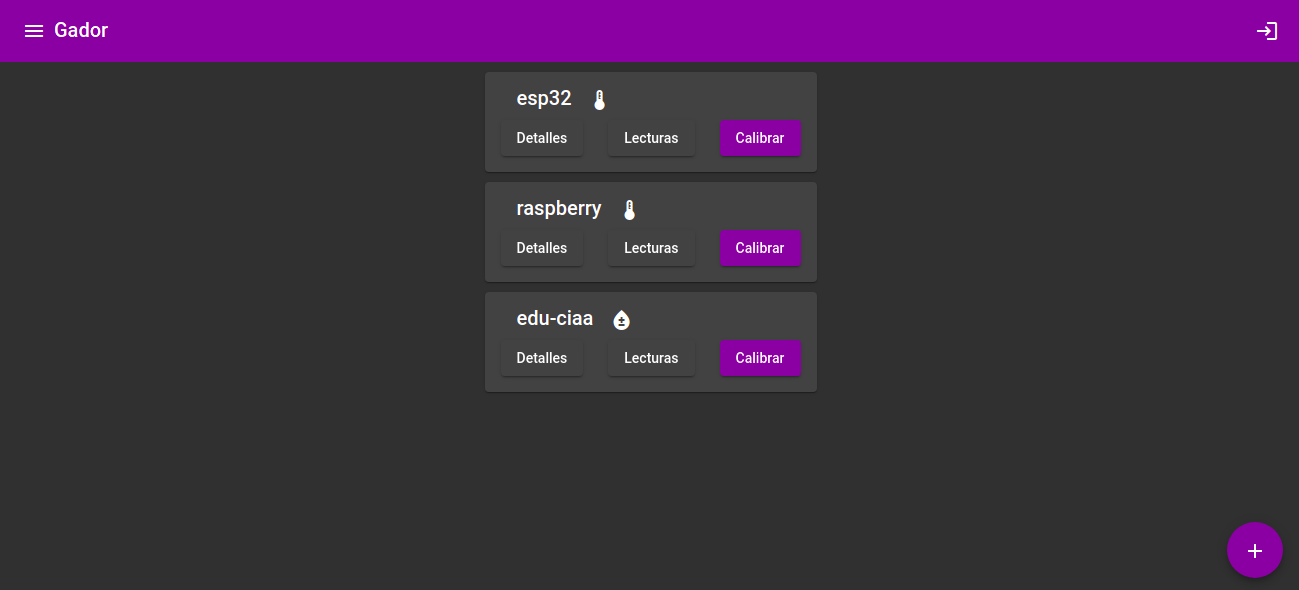
\includegraphics[width=\textwidth]{./Figures/Dispositivos.png}
	\caption{Lista de dispositivos.}
	\label{fig:ch3FrontendImg1}
\end{figure}

\begin{figure}[h]
	\centering
	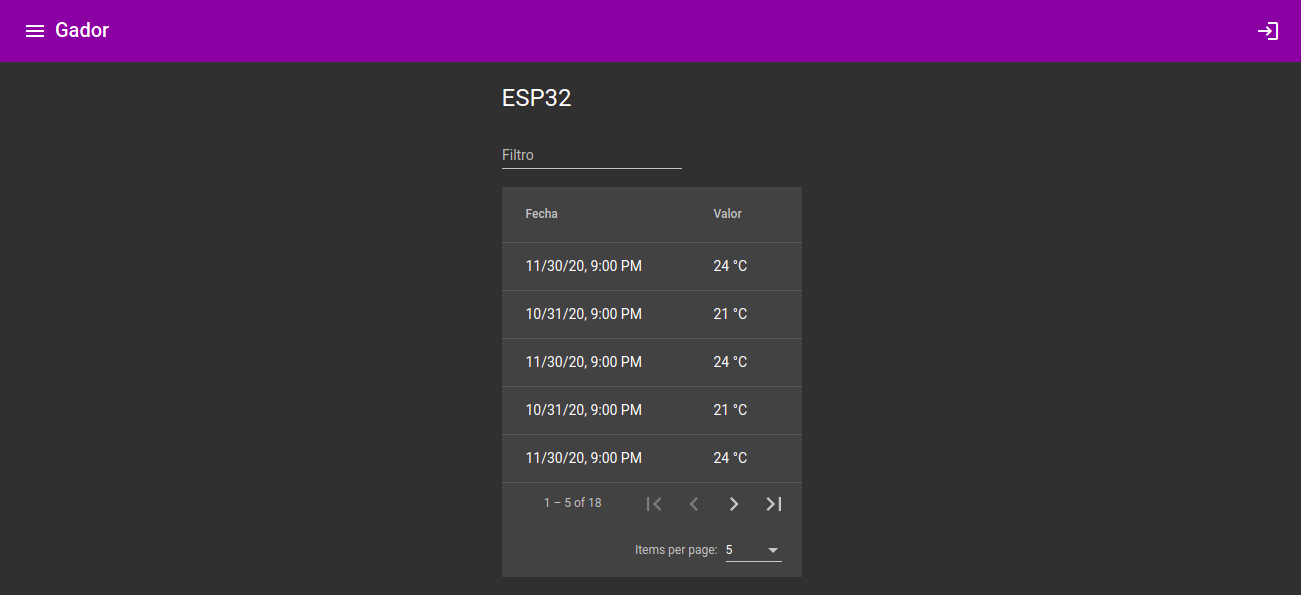
\includegraphics[width=\textwidth]{./Figures/Readings.png}
	\caption{Lecturas del sensor.}
	\label{fig:ch3FrontendImg2}
\end{figure}

\begin{figure}[h]
	\centering
	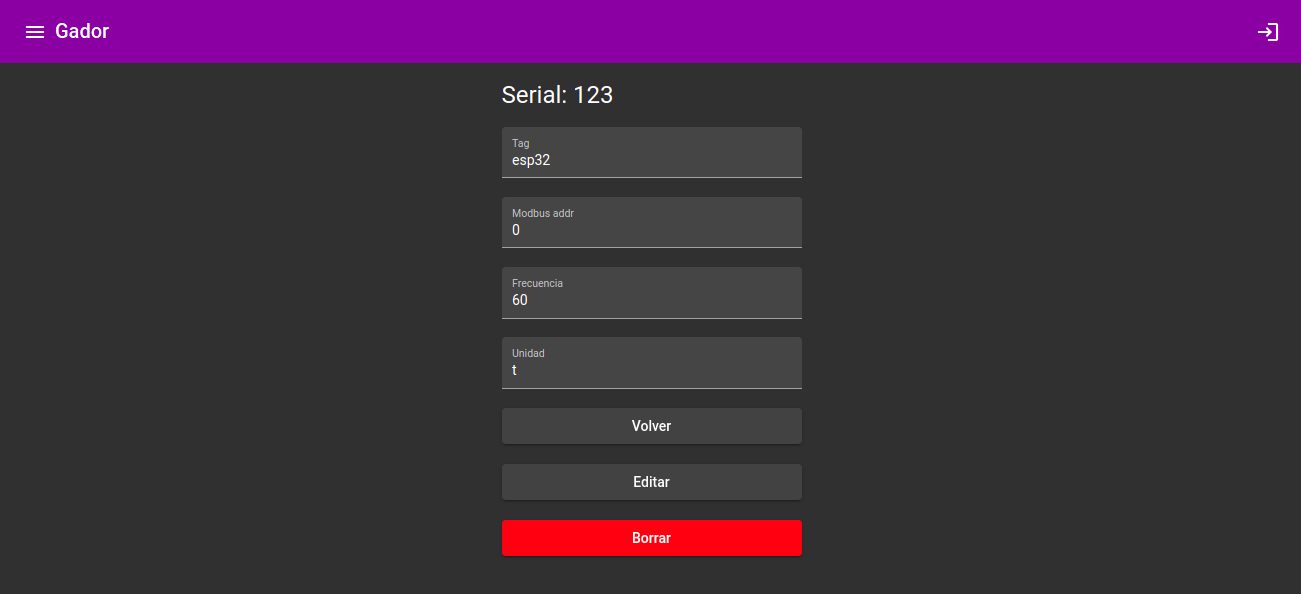
\includegraphics[width=\textwidth]{./Figures/DeviceDetails.png}
	\caption{Detalles del dispositivo.}
	\label{fig:ch3FrontendImg3}
\end{figure}